
\documentclass[11pt]{article}
\usepackage{geometry}                % See geometry.pdf to learn the layout options. There are lots.
\geometry{letterpaper}                   % ... or a4paper or a5paper or ... 
%\geometry{landscape}                % Activate for for rotated page geometry
%\usepackage[parfill]{parskip}    % Activate to begin paragraphs with an empty line rather than an indent
\usepackage{graphicx}
\usepackage{amssymb}
\usepackage{epstopdf}
\DeclareGraphicsRule{.tif}{png}{.png}{`convert #1 `dirname #1`/`basename #1 .tif`.png}

\title{Notes: Classifiers/ Discriminant Functions }
\author{Dan Beatty}
%\date{}                                           % Activate to display a given date or no date

\begin{document}
\maketitle
%\section{}
%\subsection{}

\date{1-16-2007}


\begin{quote}
One of the most useful in terms of a set of discriminant functions, $g_i(\vec{x}) , i = 1,...,c$.
\end{quote}
The purpose of discriminant functions and decision rules is to divide a feature space into $c$ decision regions, $\mathcal{R}_1,..., \mathcal{R}_c$.  Surfaces between decision regions are called decision boundaries.  

Discriminant functions assigns a feature vector to a class $\omega_i$ if $g_i (\vec{x}) > g_j (\vec{x})$ for all $j \neq i$.

Such a classifier is a network/ machine which computes $c$ discriminant functions, and selects the category corresponding to the largest discriminant.  What about a Bayes classifier?  There are two associations presented:
\begin{itemize}
	\item Assign the discriminant function to the conditional risk:
	\[
	g_i (x) = - R(\alpha_i | \vec{x})
	\]
	\item Assign the discriminant function to the posterior probability, which yields the minimal discriminant function. 
	\[
	g_i (\vec{x}) = P(\omega_i | \vec{x})
	\]
	\item The composition operator is valid on discriminant functions.  
\end{itemize}
In either case of these assignments, what derivation is this in equations 27 and 28 of Duda-Hart (page 29).  I see the application of the natural log, but it implies:
\[
\ln g_i(\vec{x}) \equiv g_i (\vec{x})
\]

\begin{eqnarray}
	g_i(x) = p(\vec{x} | \omega_i) P(\omega_i) \label{discriminantFunctionUnscaled} \\
	g_i (x) = ln p(\vec{x} | \omega_i) + ln (P(\omega_i))  \label{LnDiscriminantFunctionUnscaled}
\end{eqnarray}


The other assignment in equation \ref{discriminantFunctionUnscaled} implies that the denominator in equation 26 is equivalent to one for which I am not seeing where that scaling is either allowed or derived.  

What many have pointed out about equations \ref{discriminantFunctionUnscaled} and \ref{LnDiscriminantFunctionUnscaled} is the following:
The $g_i(\vec{x}) \to P(\omega_i | \vec{x})$ and $h_i(\vec{x}) \to p(\vec{x}|\omega_i)P(\omega_i)$ both increase in the same monotonic fashion.  Therefore, $g_i$ and $h_i$ are said to be the same discriminant function.   Likewise, $g_i$ is always positive and between 0 and 1.   Therefore $ln(g_i(\vec{x}))$ and $g_i(\vec{x})$ both point to the same discriminant function, even they are not algebraically equivalent.  

There is a diagram in \cite[30]{duda-hart-stork} shown also in this document


\begin{figure}[htbp] %  figure placement: here, top, bottom, or page
   \centering
   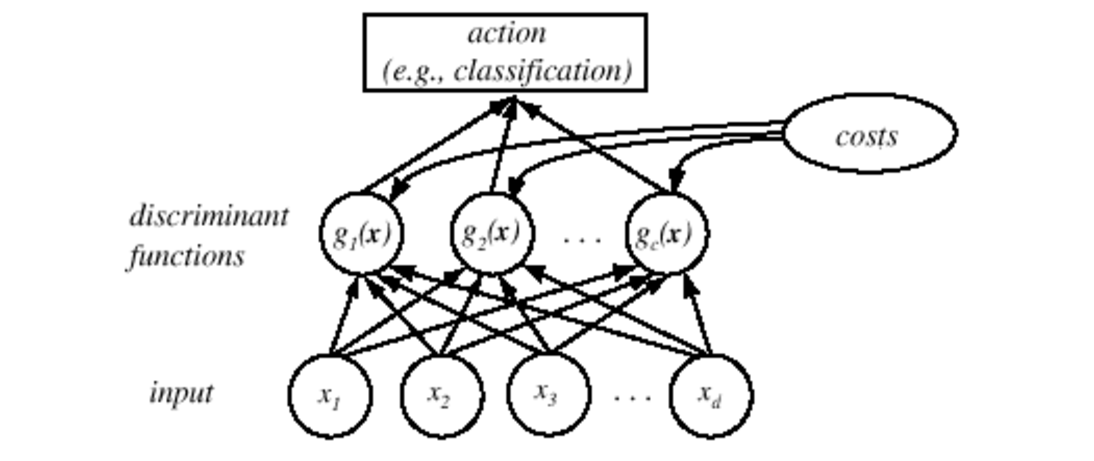
\includegraphics[width=4in]{classifiersDiagramDiscriminantFunction.pdf} 
   \caption{Classifier Discriminant Function Diagram from a functional point of view.}
   \label{fig:example}
\end{figure}

Bayes discriminant functions may be written in a variety of forms such that the decision rules are equivalent.  

Also introduced in these equations is an operator $\mathcal{R}_j$.  This operator assigns the random variable (vector) to $\omega_j$.

\subsection{Two Category Case:}
The two category case is a special cate of the multi-category case.  A dichotomizer is a classifier that consists of two categories, and places patterns into one of two categories.    The generalized method of dichotomizer would be 
\[
\left\{
\begin{array}{ll}
\vec{x} \to \omega_1  &    g_1 > g_2 \\
\vec{x} \to \omega_2  &    \textrm{ otherwise }
\end{array}
\right.
\]

Instead a dichotomizer can be reduced to 
\[
	g(\vec{x}) = P(\omega_1 | \vec{x}) - P(\omega_2 | \vec{x})
\]


\bibliography{../patternNotes}
\end{document}
